\subsection{Распределенные в пространстве ансамбли}

Понятно, что решеточные модели удобны для изучения, но, к сожалению, большинство неупорядоченных сред не имеют решеточной структуры, и требуется другой подход в изучении протекающих процессов в неупорядоченных средах. Континуальная перколяция имеет три наиболее популярные формулировки: модель пустот или модель швейцарского сыра, проблема сфер или обратная модель швейцарского сыра, модель потенциалов. Суть модели швейцарского сыра в том, что сферические пустоты (могут быть как одинакового размера, так и с некоторым распределением размеров) случайным образом помещаются внутрь проводящей среды. Сферические пустоты могут перекрывать друг друга. При критической доле объема таких пустот возникает кластер, соединяющий эти пустоты и, таким образом, среда становится непроводящей \cite{tarasevich}. Данные модели широко используются для описания транспорта в пористых средах. 

В обратной модели швейцарского сыра (проблеме сфер) рассмотрены проводящие сферы, находящиеся в непроводящей среде. Аналогично первой модели, при критическом доле объема таких сфер возникает
проводящий кластер. Модель была использована для описания прыжковой проводимости в допированных полупроводниках \cite{schlovsky} и фазовых
переходов в ферромагнетиках \cite{abrikosov}. 

\subsubsection{Случайно распределенные ансамбли}
Для расположения элементов случайным образом используются несколько различнх подходов. В данной работе рассмотрены метод Монте-Карло а также метод случайных блужданий.

Рассмотрим сначала метод Монте-Карло и его адаптацию к задаче генерации поля с ансамблем случайно-распределенных элементов.
Обобщённый алгоритм упаковки элементов выглядит следующим образом:
\begin{enumerate}
    \item Координаты центра первого элемента генерируются и записываются в массивы координат, а элементу присваивается номер $i=1$.
    \item Для каждого следующего элемента  генерируются координаты центра.
    \item Проверяется, есть ли в области, равной удвоенному характерному размеру генерируемых элементов, какие-либо генерируемые ранее элементы.
    \item Если такие находятся, то идет проверка на пересекаемость нового элемента с каждым элементом находящимся в этой области.
    \item Если сфера пересекается с какой-либо из таких сфер, она отвергается: $i$ остается прежним и переходим ко второму пункту.
    \item Если сфера не пересекается с какой-либо из таких элементов, она принимается: ее координаты записываются в массивы, элементу присваивается номер $i$.
    \item И так далее до тех пор, пока $i$ не станет равным $n$. 
\end{enumerate}

Однако данный алгоритм обладает значительным ограничением при генерации области на текущих вычислительных мощностях. Для генерации области с заданной плотностью заполненности элементами больше 50-ти процентов, время такой генерации значительно превышает время, которое можно получить альтернативными методами. Лучшим альтернативным методом является разработанный метод случайных блужданий:
\begin{enumerate}
    \item Выбирается некоторая сетка, на которой генерируются элементы в пространстве.
    \item Для каждого элемента генерируются объект с заранее заданными параметрами.
    \item Для каждого элемента производится попытка сместить элемент относительно предыдущего положения (для первого шага предыдущее положение - это положение на узлах сетки).
    \item Проверяется, есть ли в области, равной удвоенному характерному размеру генерируемых элементов, какие-либо генерируемые ранее элементы.
    \item Если такие находятся, то идет проверка на пересекаемость нового элемента с каждым элементом находящимся в этой области.
    \item Если элемент пересекается с каким-либо из таких элементов, он отвергается: $i$ остается прежним и переходим ко второму пункту.
    \item Если элемент не пересекается с каким-либо из таких элементов, он принимается: его координаты записываются в массивы, элементу присваивается номер $i$.
    \item И так далее до тех пор, пока $current_shuffle_count$ не станет равным $shuffle_count$. 
\end{enumerate}
Данный метод позволяет добиться большей плотности элементов. Максимальная плотно

\subsubsection{\label{subsubsect:tight_packing}Плотнейшая упаковка}

Термин плотнейшая упаковка характеризует специфическое расположение элементов в пространстве или на поверхности таким образом, чтобы отношение заполненной области к незаполненной было максимальным. 

При рассмотрении упаковок дисков на поверхности легко определить, что расположение сфер в центрах квадратной решётки с диаметром равным стороне данной решётки не является плотнейшим методом расположения данных элементов.

Плотнейшие упаковки в кристаллографии -- формы расположения атомов в кристаллической решётке, которые характеризуются наибольшим числом атомов в единице объёма кристалла. Такие упаковки отчётливо выражены в большом числе кристаллических структур. Они характерны для большинства металлов, а также для кристаллизованных инертных газов. Структуры многих неорганических (ионных) кристаллов представляют собой плотнейшие упаковки шаровых анионов (с большими ионными радиусами), в пустотах которых распределяются мелкие катионы.

Более 300 лет известна (И. Кеплер) и признаётся наиболее плотной упаковка шаров «вручную», когда на слой шаров, уложенных по углам квадратной сетки, наложен другой такой же слой шаров в лунки нижележащего (коэффициент заполнения пространства таким образом $74,05\%$).

\begin{figure}[h]
    \begin{subfigure}{0.49\textwidth}
        \begin{center}
            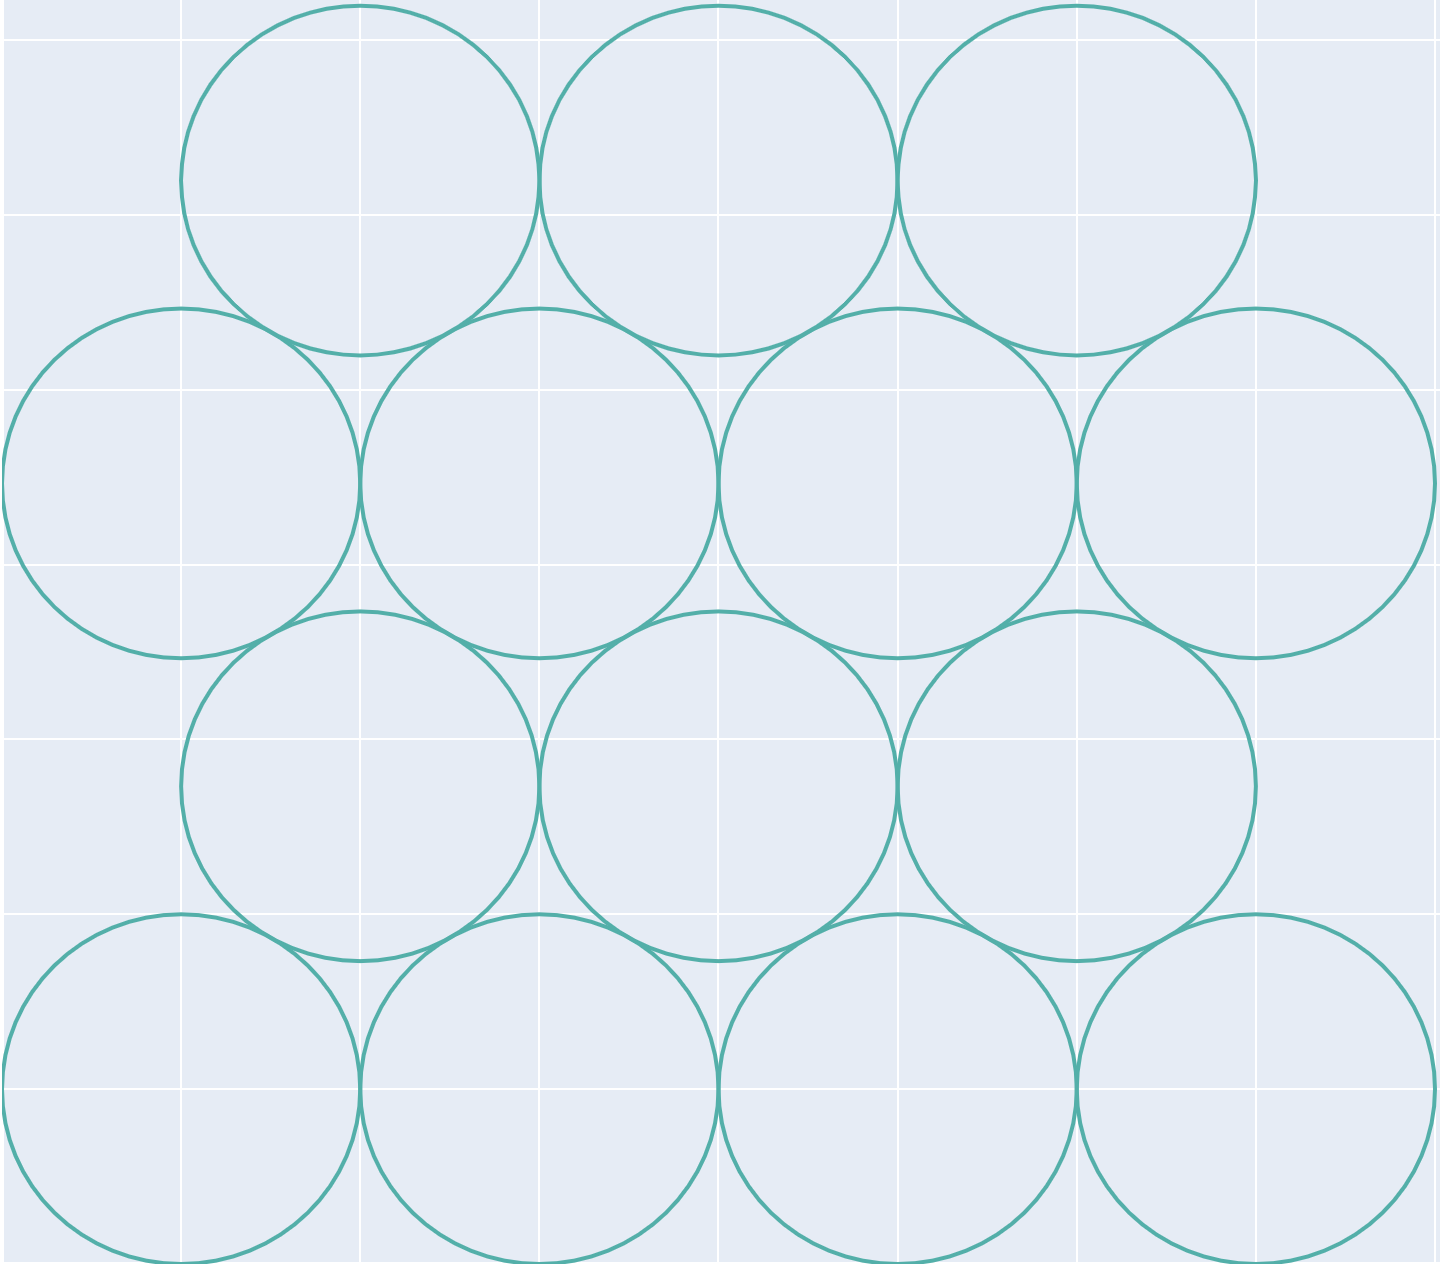
\includegraphics
            [width=8cm,height=8cm]
            {figures/circles_tighest_packing.png} 
        \end{center}
        \caption{\label{fig:tighest_circles}
        Плотнейшая упаковка окружностей}
    \end{subfigure}
    \begin{subfigure}{0.49\textwidth}
        \begin{center}
            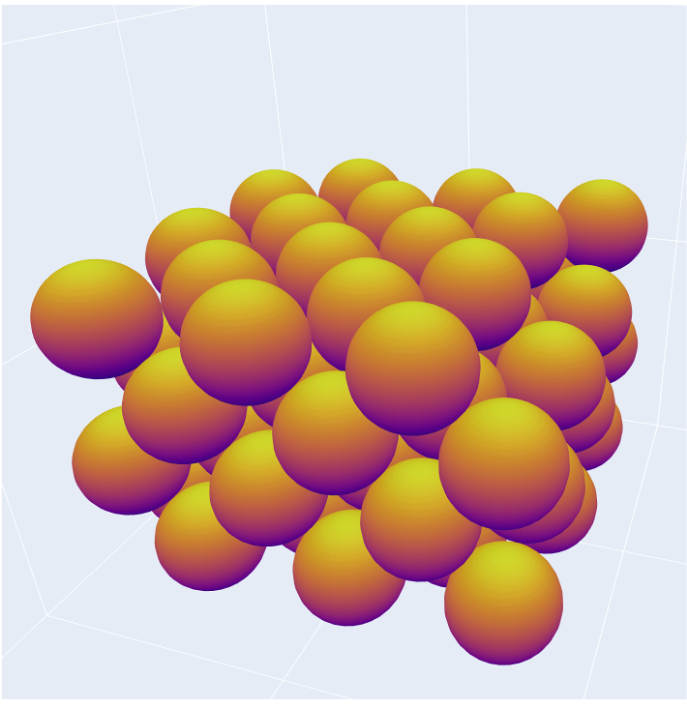
\includegraphics
            [width=8cm,height=8cm] 
            {figures/spheres_tighest_packing.png}
        \end{center}
        \caption{\label{fig:tighest_spheres}
        Плотнейшая упаковка сфер}
    \end{subfigure}
\caption{
\label{fig:main_figure}
Пример плотнейшей упаковки.
}
\end{figure}

Очевидно, что шары третьего слоя будут лежать точно над шарами первого. Такая упаковка обычно называется кубической плотнейшей гранецентрированной. Она считалась единственной, пока в 1900 английский кристаллограф У. Барлоу не показал, что, поставив куб на угол, его можно разобрать на плоские ещё более плотные слои, в которых лунок между шарами в два раза больше числа самих шаров. Варьируя укладку плотноупакованных слоев, получают бесчисленное множество плотнейших упаковок с одинаковым коэффициентом заполнения – $74,05\%$. Если ограничить наслаивание некоторым периодом, то получается: двухслойная плотнейшая упаковка, трёхслойная, четырёхслойная и так далее. Трёхслойная упаковка – это исходная кубическая, прочие – все гексагональные.

